
\documentclass[a4paper,11pt]{article}
\usepackage[a4paper, margin=8em]{geometry}

% usa i pacchetti per la scrittura in italiano
\usepackage[french,italian]{babel}
\usepackage[T1]{fontenc}
\usepackage[utf8]{inputenc}
\frenchspacing 

% usa i pacchetti per la formattazione matematica
\usepackage{amsmath, amssymb, amsthm, amsfonts}

% usa altri pacchetti
\usepackage{gensymb}
\usepackage{hyperref}
\usepackage{standalone}

\usepackage{colortbl}

\usepackage{xstring}
\usepackage{karnaugh-map}

% imposta il titolo
\title{Electronics for Embedded Systems notes}
\author{Luca Seggiani}
\date{2026}

% spaziatura liste
\usepackage{enumitem}
\setlist[itemize]{noitemsep, topsep=4pt, partopsep=0pt, parsep=2pt, leftmargin=*}
\setlist[enumerate]{noitemsep, topsep=4pt, partopsep=0pt, parsep=2pt, leftmargin=*}

% imposta lo stile
% usa helvetica
\usepackage[scaled]{helvet}
% usa palatino
\usepackage{palatino}
% usa un font monospazio guardabile
\usepackage{lmodern}

\renewcommand{\rmdefault}{ppl}
\renewcommand{\sfdefault}{phv}
\renewcommand{\ttdefault}{lmtt}

% circuiti
\usepackage{circuitikz}
\usetikzlibrary{babel}

% testo cerchiato
\newcommand*\circled[1]{\tikz[baseline=(char.base)]{
            \node[shape=circle,draw,inner sep=2pt] (char) {#1};}}

% disponi il titolo
\makeatletter
\renewcommand{\maketitle} {
	\begin{center} 
		\begin{minipage}[t]{.8\textwidth}
			\textsf{\huge\bfseries \@title} 
		\end{minipage}%
		\begin{minipage}[t]{.2\textwidth}
			\raggedleft \vspace{-1.65em}
			\textsf{\small \@author} \vfill
			\textsf{\small \@date}
		\end{minipage}
		\par
	\end{center}

	\thispagestyle{empty}
	\pagestyle{fancy}
}
\makeatother

% disponi teoremi
\usepackage{tcolorbox}
\newtcolorbox[auto counter, number within=section]{theorem}[2][]{%
	colback=blue!10, 
	colframe=blue!40!black, 
	sharp corners=northwest,
	fonttitle=\sffamily\bfseries, 
	title=Theorem~\thetcbcounter: #2, 
	#1
}

% disponi definizioni
\newtcolorbox[auto counter, number within=section]{definition}[2][]{%
	colback=red!10,
	colframe=red!40!black,
	sharp corners=northwest,
	fonttitle=\sffamily\bfseries,
	title=Definition~\thetcbcounter: #2,
	#1
}

% disponi codice
\usepackage{listings}
\usepackage[table]{xcolor}

\definecolor{codegreen}{rgb}{0,0.6,0}
\definecolor{codegray}{rgb}{0.5,0.5,0.5}
\definecolor{codepurple}{rgb}{0.58,0,0.82}
\definecolor{backcolour}{rgb}{0.95,0.95,0.92}

\lstdefinestyle{codestyle}{
		backgroundcolor=\color{black!5}, 
		commentstyle=\color{codegreen},
		keywordstyle=\bfseries\color{magenta},
		numberstyle=\sffamily\tiny\color{black!60},
		stringstyle=\color{green!50!black},
		basicstyle=\ttfamily\footnotesize,
		breakatwhitespace=false,         
		breaklines=true,                 
		captionpos=b,                    
		keepspaces=true,                 
		numbers=left,                    
		numbersep=5pt,                  
		showspaces=false,                
		showstringspaces=false,
		showtabs=false,                  
		tabsize=2
}

\lstdefinestyle{shellstyle}{
		backgroundcolor=\color{black!5}, 
		basicstyle=\ttfamily\footnotesize\color{black}, 
		commentstyle=\color{black}, 
		keywordstyle=\color{black},
		numberstyle=\color{black!5},
		stringstyle=\color{black}, 
		showspaces=false,
		showstringspaces=false, 
		showtabs=false, 
		tabsize=2, 
		numbers=none, 
		breaklines=true
}

\lstdefinelanguage{x86}{ 
  keywords={AAA, AAD, AAM, AAS, ADC, ADCB, ADCW, ADCL, ADD, ADDB, ADDW, ADDL, AND, ANDB, ANDW, ANDL,
        ARPL, BOUND, BSF, BSFL, BSFW, BSR, BSRL, BSRW, BSWAP, BT, BTC, BTCB, BTCW, BTCL, BTR, 
        BTRB, BTRW, BTRL, BTS, BTSB, BTSW, BTSL, CALL, CBW, CDQ, CLC, CLD, CLI, CLTS, CMC, CMP,
        CMPB, CMPW, CMPL, CMPS, CMPSB, CMPSD, CMPSW, CMPXCHG, CMPXCHGB, CMPXCHGW, CMPXCHGL,
        CMPXCHG8B, CPUID, CWDE, DAA, DAS, DEC, DECB, DECW, DECL, DIV, DIVB, DIVW, DIVL, ENTER,
        HLT, IDIV, IDIVB, IDIVW, IDIVL, IMUL, IMULB, IMULW, IMULL, IN, INB, INW, INL, INC, INCB,
        INCW, INCL, INS, INSB, INSD, INSW, INT, INT3, INTO, INVD, INVLPG, IRET, IRETD, JA, JAE,
        JB, JBE, JC, JCXZ, JE, JECXZ, JG, JGE, JL, JLE, JMP, JNA, JNAE, JNB, JNBE, JNC, JNE, JNG,
        JNGE, JNL, JNLE, JNO, JNP, JNS, JNZ, JO, JP, JPE, JPO, JS, JZ, LAHF, LAR, LCALL, LDS,
        LEA, LEAVE, LES, LFS, LGDT, LGS, LIDT, LMSW, LOCK, LODSB, LODSD, LODSW, LOOP, LOOPE,
        LOOPNE, LSL, LSS, LTR, MOV, MOVB, MOVW, MOVL, MOVSB, MOVSD, MOVSW, MOVSX, MOVSXB,
        MOVSXW, MOVSXL, MOVZX, MOVZXB, MOVZXW, MOVZXL, MUL, MULB, MULW, MULL, NEG, NEGB, NEGW,
        NEGL, NOP, NOT, NOTB, NOTW, NOTL, OR, ORB, ORW, ORL, OUT, OUTB, OUTW, OUTL, OUTSB, OUTSD,
        OUTSW, POP, POPL, POPW, POPB, POPA, POPAD, POPF, POPFD, PUSH, PUSHL, PUSHW, PUSHB, PUSHA, 
        RCLL, RCR, RCRB, RCRW, RCRL, RDMSR, RDPMC, RDTSC, REP, REPE, REPNE, RET, ROL, ROLB, ROLW,
        ROLL, ROR, RORB, RORW, RORL, SAHF, SAL, SALB, SALW, SALL, SAR, SARB, SARW, SARL, SBB,
        SBBB, SBBW, SBBL, SCASB, SCASD, SCASW, SETA, SETAE, SETB, SETBE, SETC, SETE, SETG, SETGE,
        SETL, SETLE, SETNA, SETNAE, SETNB, SETNBE, SETNC, SETNE, SETNG, SETNGE, SETNL, SETNLE,
        SETNO, SETNP, SETNS, SETNZ, SETO, SETP, SETPE, SETPO, SETS, SETZ, SGDT, SHL, SHLB, SHLW,
        SHLL, SHLD, SHR, SHRB, SHRW, SHRL, SHRD, SIDT, SLDT, SMSW, STC, STD, STI, STOSB, STOSD,
        STOSW, STR, SUB, SUBB, SUBW, SUBL, TEST, TESTB, TESTW, TESTL, VERR, VERW, WAIT, WBINVD,
        XADD, XADDB, XADDW, XADDL, XCHG, XCHGB, XCHGW, XCHGL, XLAT, XLATB, XOR, XORB, XORW, XORL},
  keywordstyle=\color{blue}\bfseries,
  ndkeywordstyle=\color{darkgray}\bfseries,
  identifierstyle=\color{black},
  sensitive=false,
  comment=[l]{\#},
  morecomment=[s]{/*}{*/},
  commentstyle=\color{purple}\ttfamily,
  stringstyle=\color{red}\ttfamily,
  morestring=[b]',
  morestring=[b]"
}

\lstdefinelanguage{riscv}{
  keywords={
    LUI, AUIPC,
    JAL, JALR,
    BEQ, BNE, BLT, BGE, BLTU, BGEU,
    LB, LH, LW, LBU, LHU, LD,
    SB, SH, SW, SD,
    ADDI, SLTI, SLTIU, XORI, ORI, ANDI,
    SLLI, SRLI, SRAI,
    ADD, SUB, SLL, SLT, SLTU, XOR, SRL, SRA, OR, AND,
    ADDIW, SLLIW, SRLIW, SRAIW,
    ADDW, SUBW, SLLW, SRLW, SRAW,
    MUL, MULH, MULHSU, MULHU, DIV, DIVU, REM, REMU,
    MULW, DIVW, DIVUW, REMW, REMUW,
    LR.W, SC.W, AMOSWAP.W, AMOADD.W, AMOXOR.W,
    AMOAND.W, AMOOR.W, AMOMIN.W, AMOMAX.W,
    AMOMINU.W, AMOMAXU.W,
    LR.D, SC.D, AMOSWAP.D, AMOADD.D, AMOXOR.D,
    AMOAND.D, AMOOR.D, AMOMIN.D, AMOMAX.D,
    AMOMINU.D, AMOMAXU.D,
    FLW, FSW,
    FMADD.S, FMSUB.S, FNMSUB.S, FNMADD.S,
    FADD.S, FSUB.S, FMUL.S, FDIV.S, FSQRT.S,
    FSGNJ.S, FSGNJN.S, FSGNJX.S,
    FMIN.S, FMAX.S,
    FCVT.W.S, FCVT.WU.S, FCVT.S.W, FCVT.S.WU,
    FMV.X.W, FMV.W.X,
    FEQ.S, FLT.S, FLE.S,
    FLD, FSD,
    FMADD.D, FMSUB.D, FNMSUB.D, FNMADD.D,
    FADD.D, FSUB.D, FMUL.D, FDIV.D, FSQRT.D,
    FSGNJ.D, FSGNJN.D, FSGNJX.D,
    FMIN.D, FMAX.D,
    FCVT.W.D, FCVT.WU.D, FCVT.D.W, FCVT.D.WU,
    FCVT.S.D, FCVT.D.S,
    FMV.X.D, FMV.D.X,
    FEQ.D, FLT.D, FLE.D,
    CSRRW, CSRRS, CSRRC,
    CSRRWI, CSRRSI, CSRRCI,
    FENCE.I,
    FENCE,
    ECALL, EBREAK,
    MRET, SRET, URET,
    WFI,
    SFENCE.VMA,
    NOP, LI, LA, MV,
    NOT, NEG, NEGW,
    SEQZ, SNEZ, SLTZ, SGTZ,
    BEQZ, BNEZ, BLEZ, BGEZ, BLTZ, BGTZ,
    BGT, BLE, BGTU, BLEU,
    J, JR, RET,
    CALL, TAIL,
    RDINSTRET, RDCYCLE, RDTIME,
    CSRR, CSRW, CSRS, CSRC,
    CSRWI, CSRSI, CSRCI
  },
  keywordstyle=\color{blue}\bfseries,
  ndkeywordstyle=\color{darkgray}\bfseries,
  identifierstyle=\color{black},
  sensitive=false,
  comment=[l]{\#},
  morecomment=[s]{/*}{*/},
  commentstyle=\color{purple}\ttfamily,
  stringstyle=\color{red}\ttfamily,
  morestring=[b]',
  morestring=[b]"
}

\lstdefinelanguage{arm}{
  keywords={
    ADC, ADD, AND, BIC, CMN, CMP, EOR, MOV, MVN,
    RSB, RSC, SBC, SUB, TST, TEQ,
    MLA, MLS, MUL, SMLAL, SMULL, UMLAL, UMULL,
    QADD, QSUB, QDADD, QDSUB,
    QADD16, QADD8, QASX, QSAX,
    QSUB16, QSUB8, QSAX, QSUBADDX,
    ASR, LSL, LSR, ROR, RRX,
    B, BL, BX, BLX,
    BXJ,
    BEQ, BNE, BCS, BHS, BCC, BLO,
    BMI, BPL, BVS, BVC,
    BHI, BLS, BGE, BLT, BGT, BLE,
    BAL,
    LDR, LDRB, LDRH, LDRSB, LDRSH,
    LDRD, LDM, LDMIA, LDMIB, LDMDA, LDMDB,
    LDRT, LDRBT, LDRHT, LDRSBT, LDRSHT,
    STR, STRB, STRH, STRD,
    STM, STMIA, STMIB, STMDA, STMDB,
    STRT, STRBT, STRHT,
    PUSH, POP,
    SWP, SWPB,
    REV, REV16, REVSH,
    BFC, BFI, BFXIL, SBFX, UBFX,
    CLZ,
    LDREX, LDREXB, LDREXH, LDREXD,
    STREX, STREXB, STREXH, STREXD,
    DMB, DSB, ISB,
    MCR, MCRR, MRC, MRRC,
    MRS, MSR,
    CPS, SETEND, SVC, BKPT,
    CLREX, WFE, WFI, SEV,
    YIELD, NOP,
    VLDR, VSTR,
    VMOV, VABS, VNEG,
    VADD, VSUB, VMUL, VDIV,
    VMLA, VMLS, VNMLA, VNMLS, VNMUL,
    VMAX, VMIN,
    VSQRT,
    VCMP, VCMPE,
    VCVT,
    VCLZ, VCLS,
    VAND, VORR, VEOR, VBIC, VMVN,
    VLD1, VLD2, VLD3, VLD4,
    VST1, VST2, VST3, VST4,
    ADR, ADCS, ADDS, SUBS, MOVS, ANDS, ORRS, EORS
  },
  keywordstyle=\color{blue}\bfseries,
  ndkeywordstyle=\color{darkgray}\bfseries,
  identifierstyle=\color{black},
  sensitive=false,
  comment=[l]{@},
  morecomment=[l]{;},
  morecomment=[s]{/*}{*/},
  commentstyle=\color{purple}\ttfamily,
  stringstyle=\color{red}\ttfamily,
  morestring=[b]',
  morestring=[b]"
}

\lstset{style=codestyle, language=C}

% disponi sezioni
\usepackage{titlesec}

\titleformat{\section}
	{\sffamily\Large\bfseries} 
	{\thesection}{1em}{} 
\titleformat{\subsection}
	{\sffamily\large\bfseries}   
	{\thesubsection}{1em}{} 
\titleformat{\subsubsection}
	{\sffamily\normalsize\bfseries} 
	{\thesubsubsection}{1em}{}

% tikz
\usepackage{tikz}

% float
\usepackage{float}

% grafici
\usepackage{pgfplots}
\pgfplotsset{width=10cm,compat=1.9}

% disponi alberi
\usepackage{forest}

\forestset{
	rectstyle/.style={
		for tree={rectangle,draw,font=\large\sffamily}
	},
	roundstyle/.style={
		for tree={circle,draw,font=\large}
	}
}

% disponi algoritmi
\usepackage{algorithm}
\usepackage{algorithmic}
\makeatletter
\renewcommand{\ALG@name}{Algorithm}
\makeatother

% disponi numeri di pagina
\usepackage{fancyhdr}
\fancyhf{} 
\fancyfoot[L]{\sffamily{\thepage}}

\makeatletter
\fancyhead[L]{\raisebox{1ex}[0pt][0pt]{\sffamily{\@title \ \@date}}} 
\fancyhead[R]{\raisebox{1ex}[0pt][0pt]{\sffamily{\@author}}}
\makeatother

\begin{document}
% sezione (data)
\section{Lesson 13-10-26}

% stili pagina
\thispagestyle{empty}
\pagestyle{fancy}

% testo
\subsection{Content addressable memories}

\textbf{CAM}s (\textit{Content Addressable Memories}), also known as \textit{associative memories}, are special kinds of memory where the main operation is a \textbf{match operation}.
Instead of providing the address and read the data, want to look for the \textit{address} of some given data.
This can be done in software, via indices or simple linear scans, but is far more efficient and faster (if not more expensive) to do in memory.

Let's look at the cell.

\begin{center}
	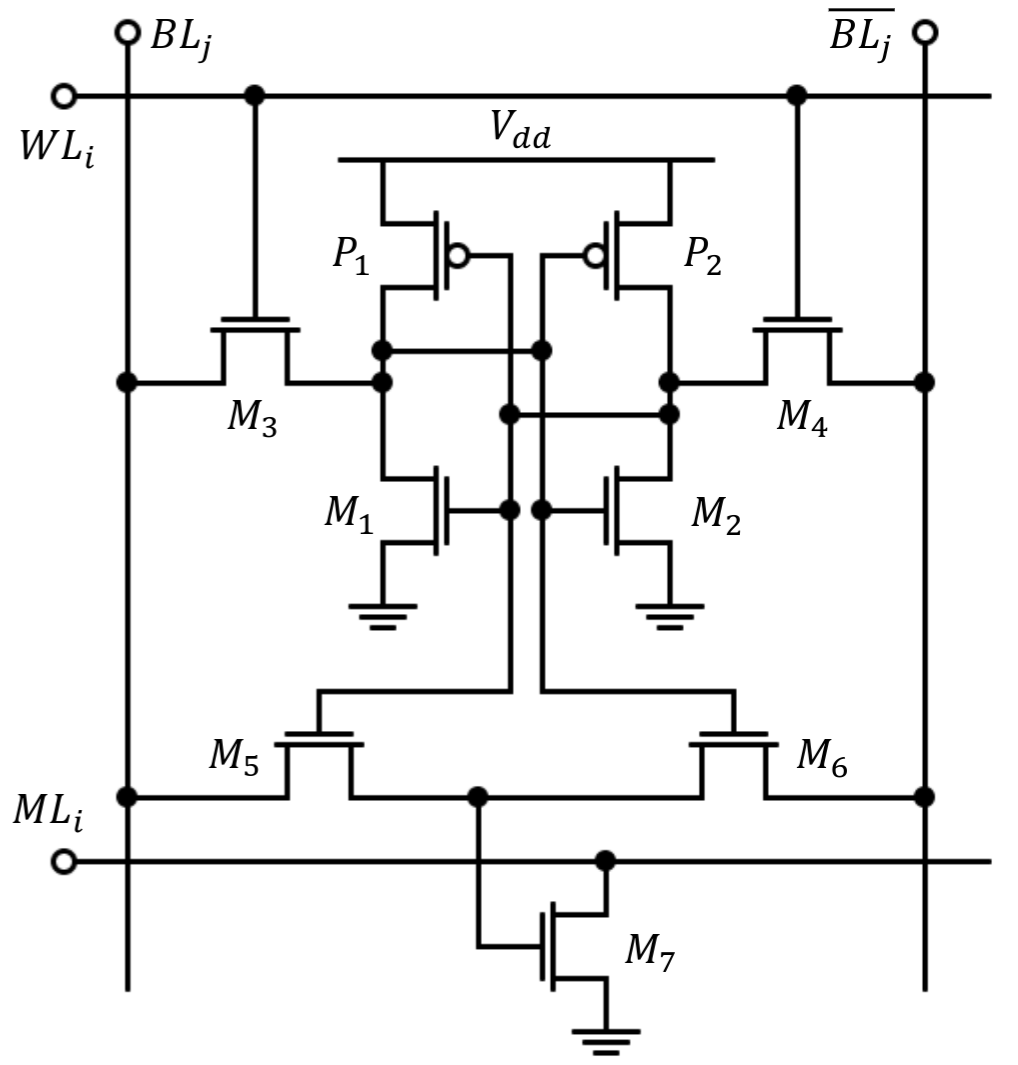
\includegraphics[scale=0.22]{../figures/cam_cell.png}
\end{center}

For the match operation, the word Line $WL_i$ remains inactive for the entire operation: we don’t want to change the bit cell content.
Instead we recharge Match Line $ML_i$ to $V_{dd}$, then apply the value to $BL_i$ and its complement to $\overline{BL_i}$.
If there is no match, $ML_i$ will be discharged.

There are 4 main cases to study here:
\begin{enumerate}
	\item Contaning 1, matching 1:
	\begin{center}
		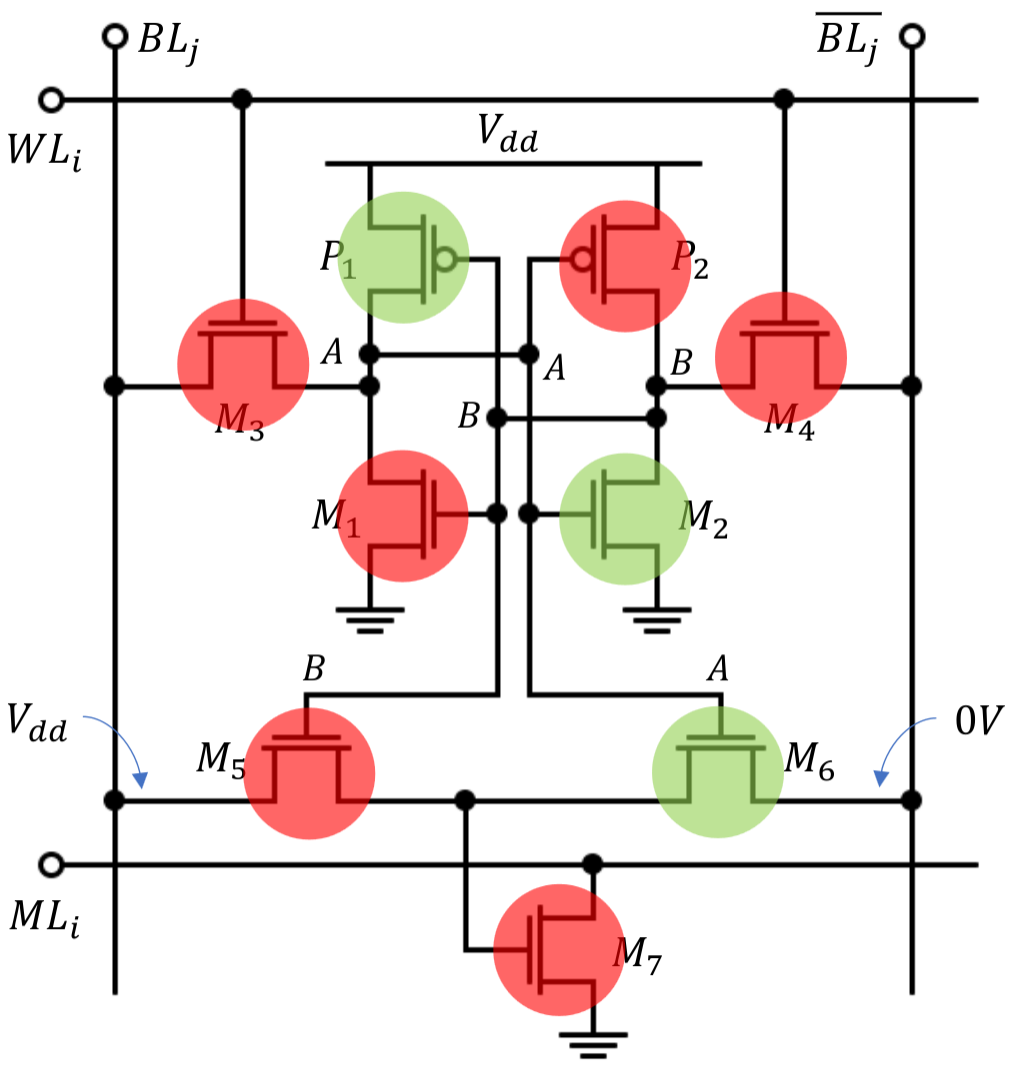
\includegraphics[scale=0.1]{../figures/cam/cam1.png}
	\end{center}
	\item Contaning 1, matching 0:
	\begin{center}
		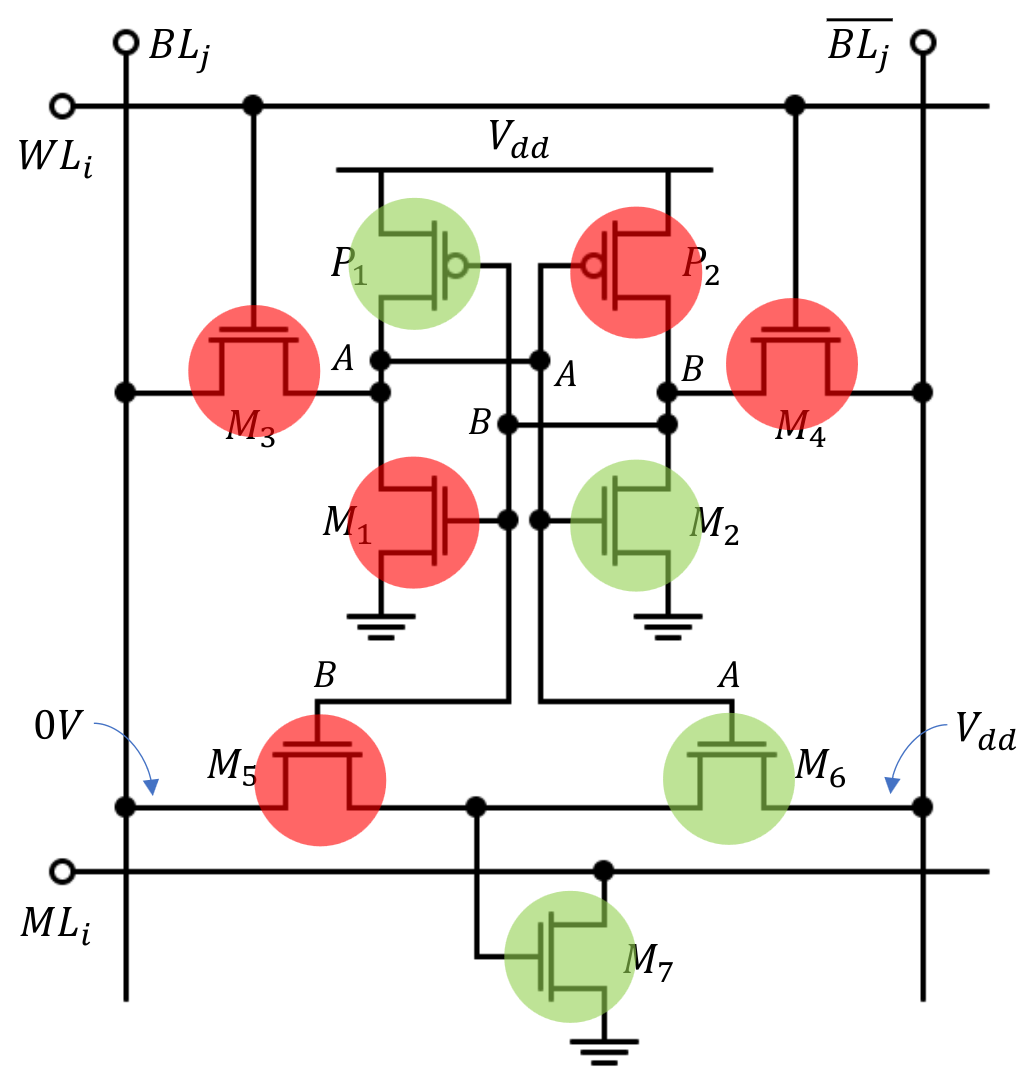
\includegraphics[scale=0.1]{../figures/cam/cam2.png}
	\end{center}
	\item Contaning 0, matching 0:
	\begin{center}
		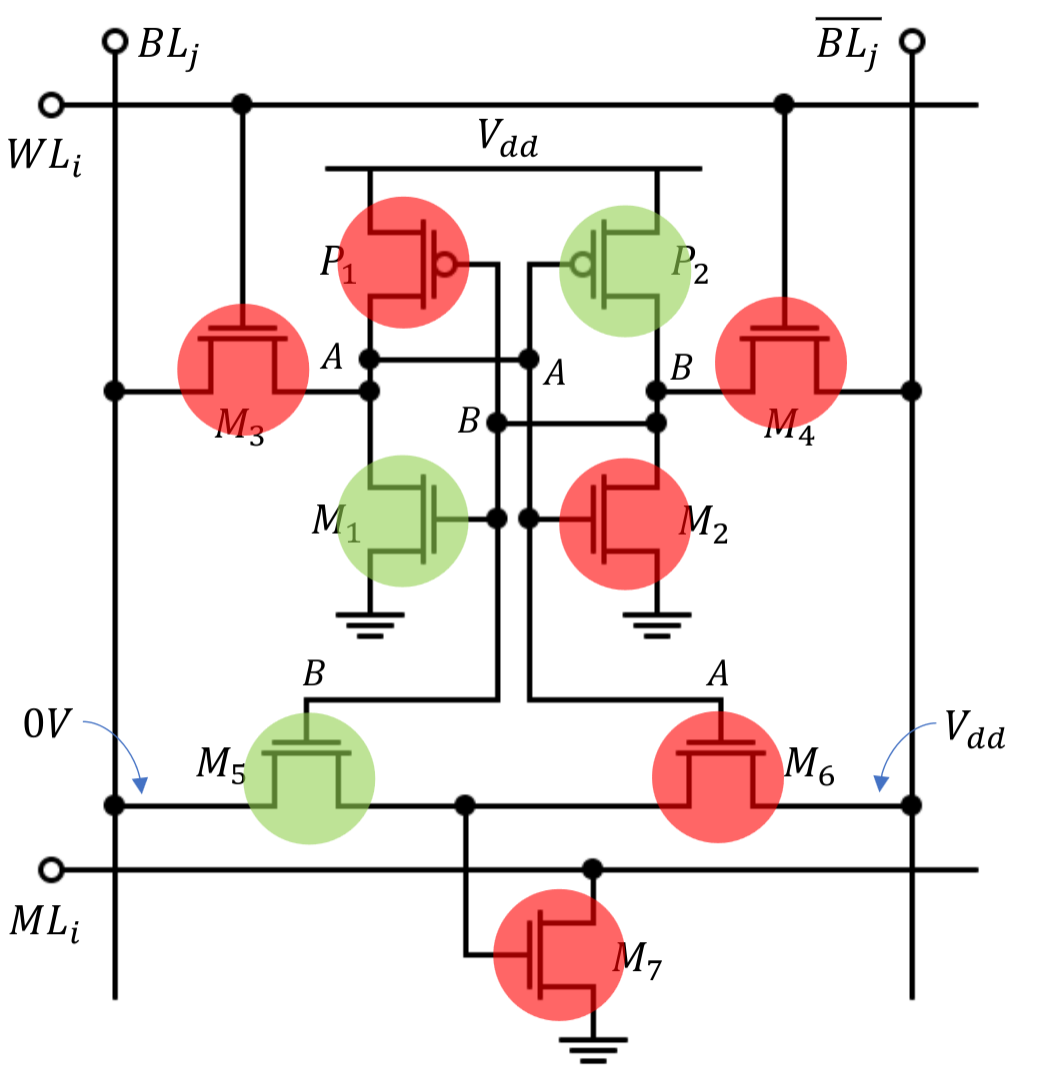
\includegraphics[scale=0.1]{../figures/cam/cam3.png}
	\end{center}
	\item Contaning 0, matching 1:
	\begin{center}
		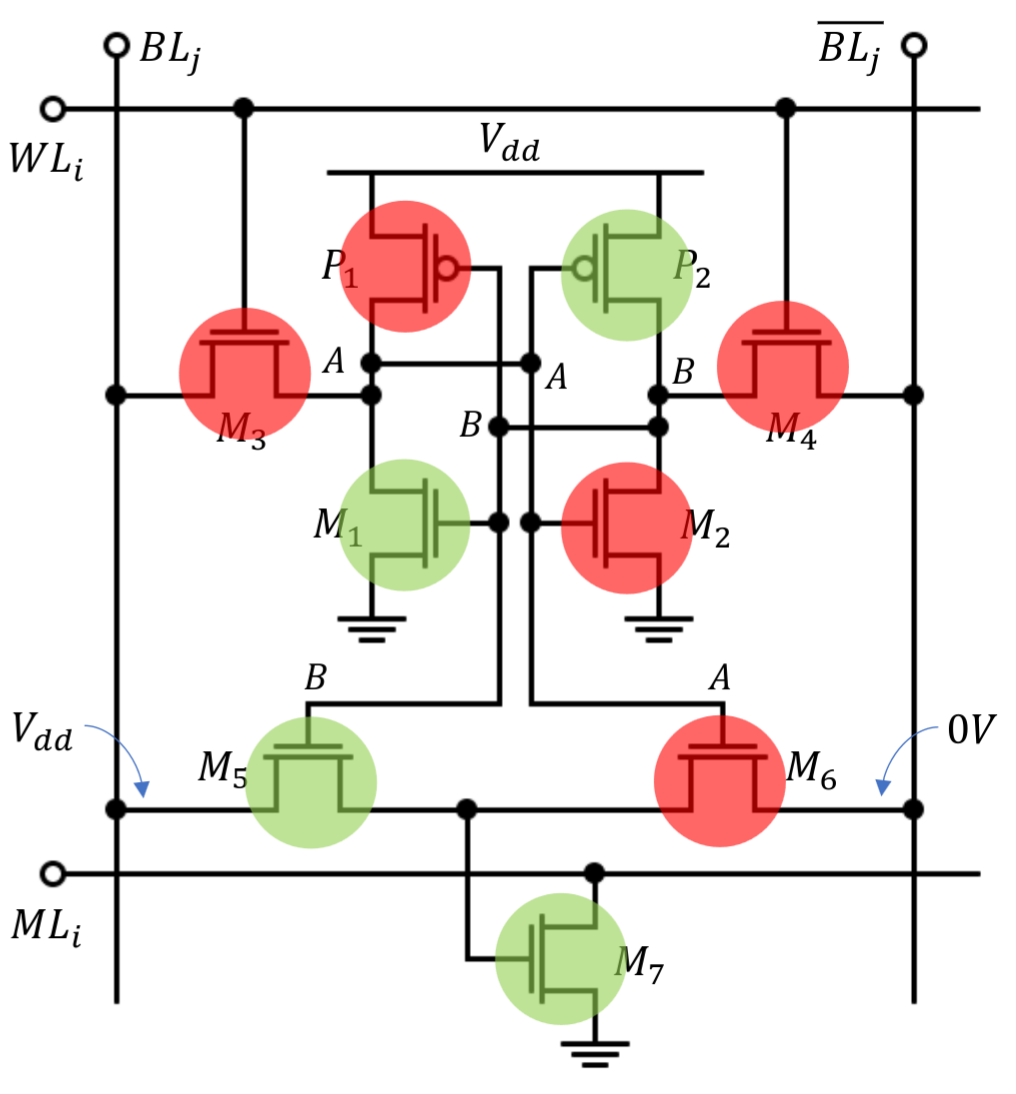
\includegraphics[scale=0.1]{../figures/cam/cam4.png}
	\end{center}
\end{enumerate}

We then have other 2 cases, which relate to the \textit{don't care} search state.
We can perform a search by not caring if we set both bit lines to 0.
\begin{enumerate}
	\item Contaning 1, don't care:
	\begin{center}
		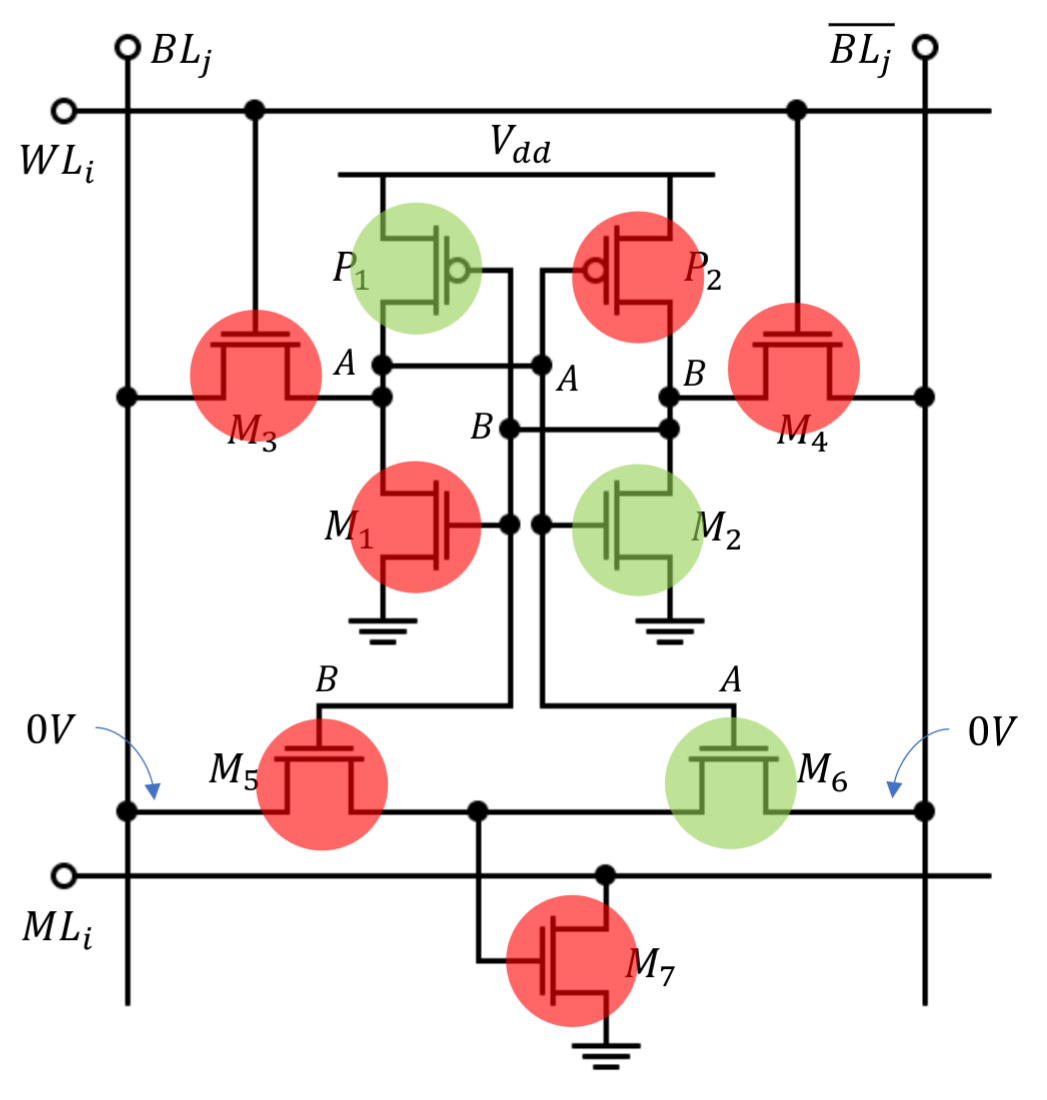
\includegraphics[scale=0.1]{../figures/cam/cam5.png}
	\end{center}
	\item Contaning 0, don't care:
	\begin{center}
		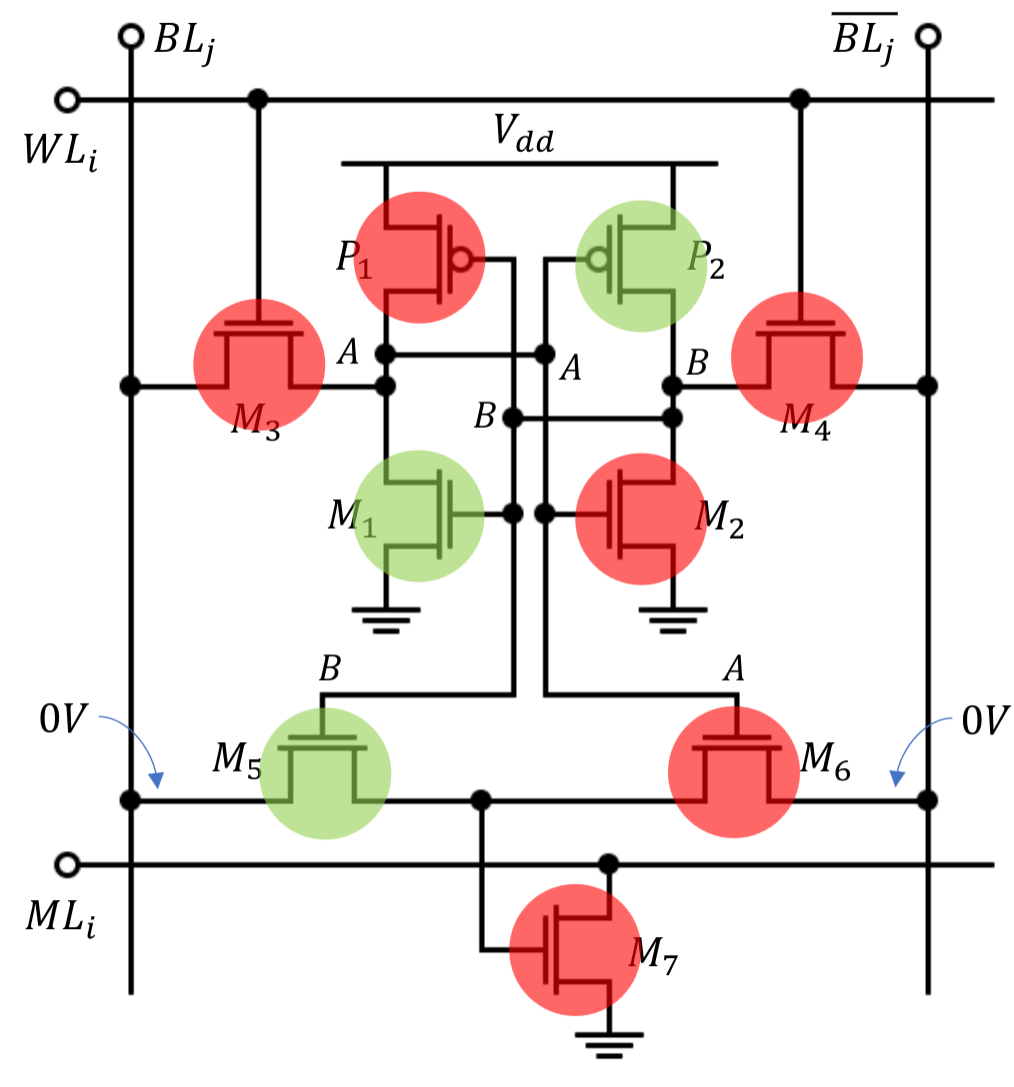
\includegraphics[scale=0.1]{../figures/cam/cam6.png}
	\end{center}
\end{enumerate}

At this point we have documented the behavoir of the CAM cell enough to look at the actual topology:
\begin{center}
	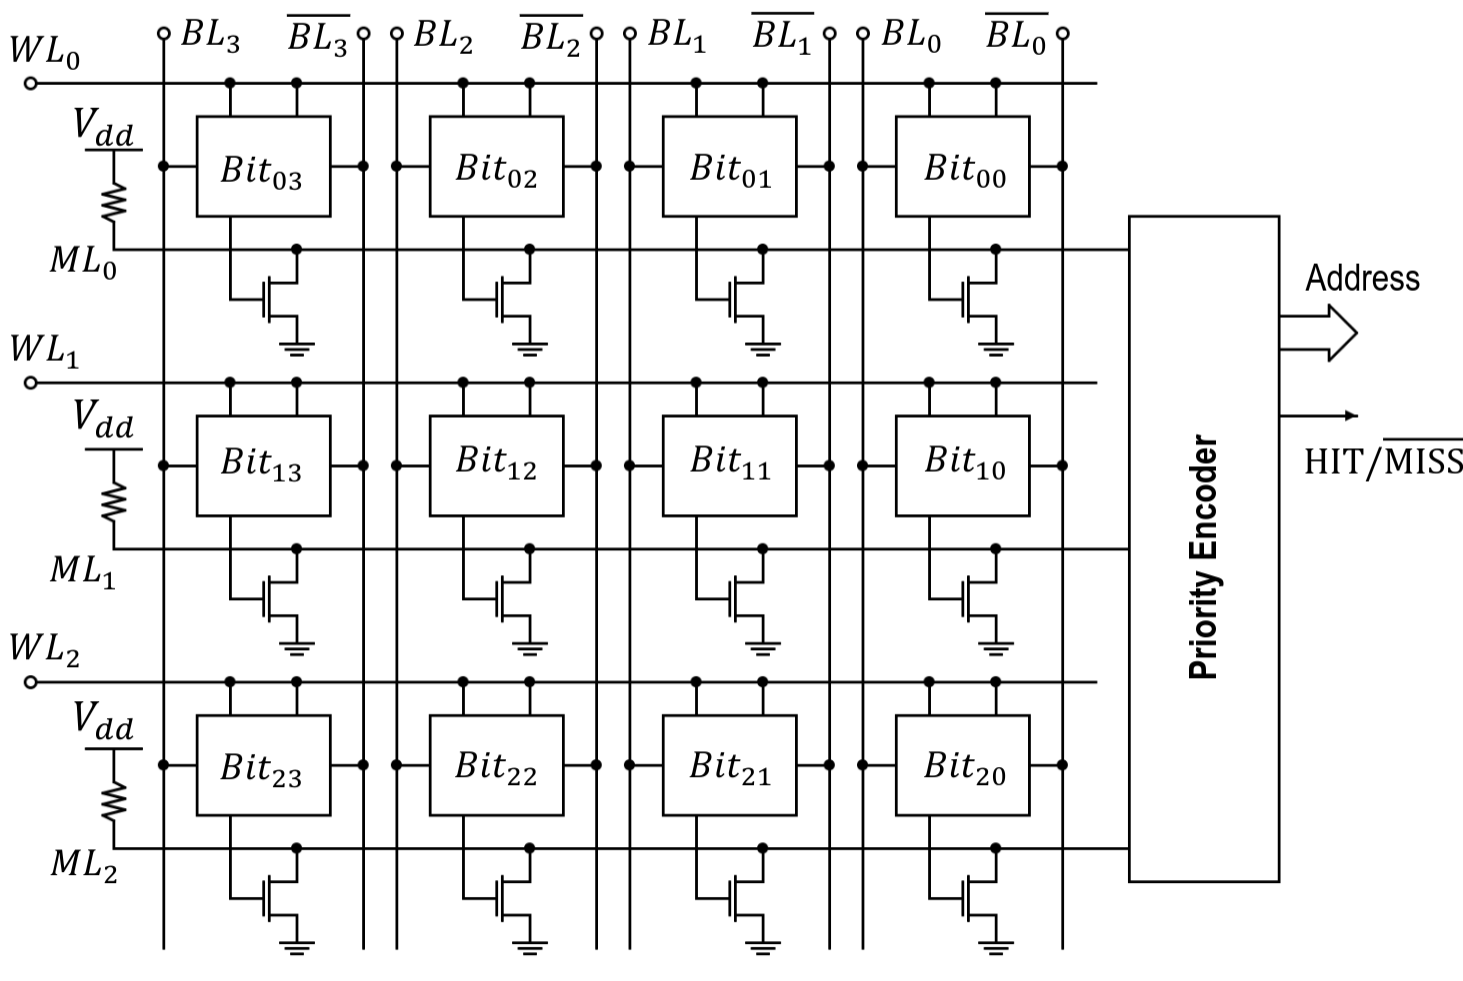
\includegraphics[scale=0.22]{../figures/cam_topo.png}
\end{center}

Note that:
\begin{itemize}
	\item Each Match Line spans an entire word, but not an entire row!
	This means that if all bits in Word $i$ match, the Match Line $ML_i$ is high. If on the other hand at least one bit in Word $i$ does not match, the Match Line $ML_i$ is low;
	\item Then note the \textit{priority encoder}. If at least one Match Line is high, the priority encoder asserts HIT, and it generates the corresponding address (the highest). On the other hand, if all Match Lines are low, the priority encoder asserts MISS.


\end{itemize}

\subsubsection{Associative SRAM}

Let's look into how an actual \textbf{associative SRAM} is built from this premise.

In the simplest case an associative SRAM is only a circuit with the topology shown in the last section. 
When such an Associative SRAM is switched ON the content is random.

Let's assume some data is written, but only partially occupies the memory: we want to match only against the written data.

To do this, we have all words in the associative memory contain an additional bit, called the \textit{valid bit}. At power on also the valid bit is also random, so a special associative memory operation initializes all valid bits to 0.
This means marking all words as invalid

When writing a word, the corresponding valid bit is automatically set.
At this point, when matching, all valid bits are automatically matched against logic 1, whereas all invalid words do not match.

\subsubsection{Associative SRAM performance}

Doing matchin in hardware means all matching performed in parallel, which is much better than scanning the entire memory sequentially.
This makes for a very quick result (tens of nanoseconds).

Of course, because of increased parasitic capacitances, the larger the memory, the slower the matching.

It goes without saying that such a ram is more expensive than an SRAM, with 9 transistors compared to 6 transistors for a single cell.
The bit cell is also larger, has high power consumption, and especially high power consumption during the match operation (we have to precharge all match lines, only to discharge most (or all) of them).

\subsubsection{Ternary CAM}

There is another kind of CAM, which allows for \textit{don't care} states to be encoded directly in the memory.

\begin{center}
	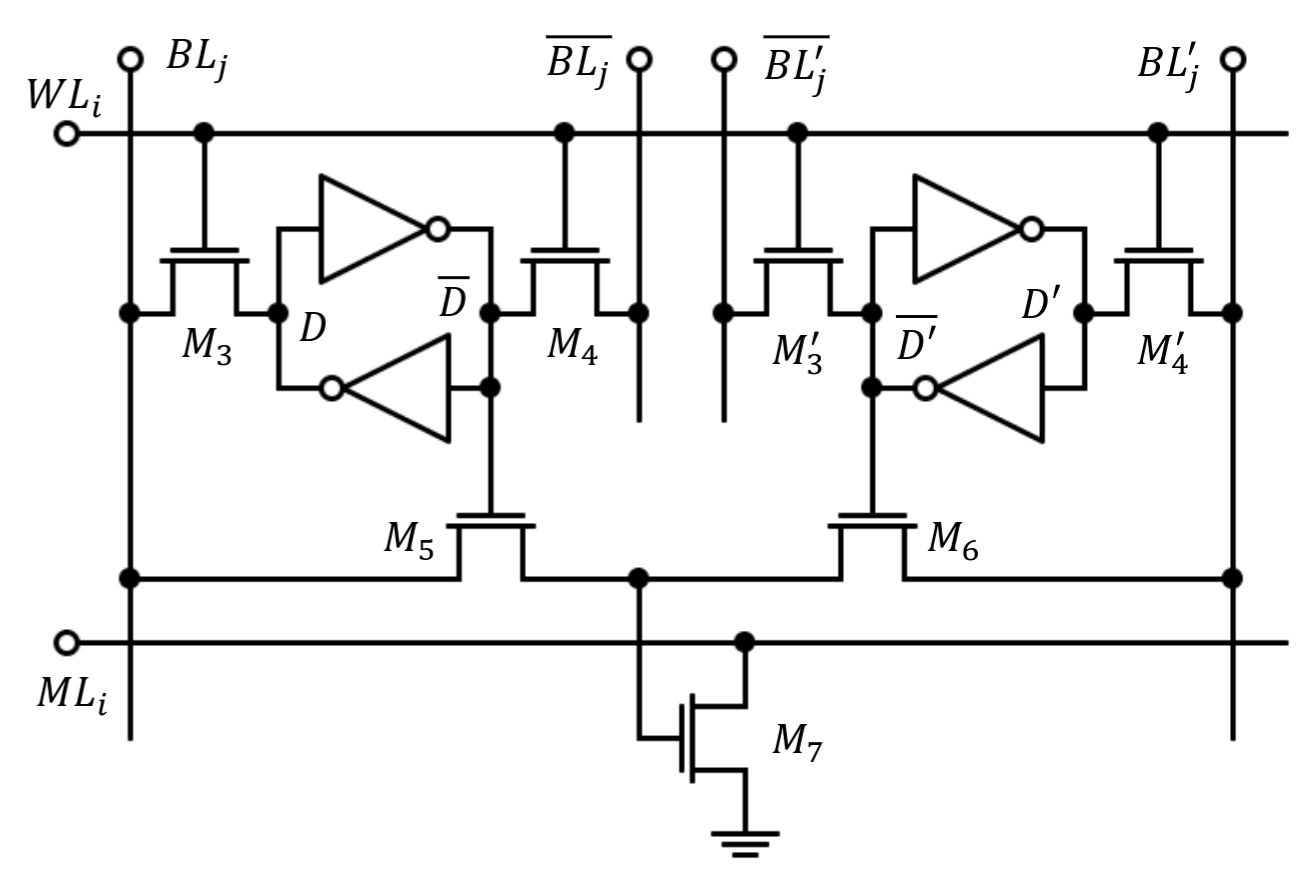
\includegraphics[scale=0.2]{../figures/ternary_cam.png}
\end{center}

To do this we have two bit cells for each bit in the memory.
We map the usual \texttt{10} and \texttt{01} values to logic 1 and 0 (same as normal SRAM), but also reserve \texttt{11} for don't care.

Matching can be done the same, as searching for \texttt{00} when the actual value is \texttt{11} keeps the $ML_i$ high.

This kind of memory is really useful in \textit{routers}, where routing tables often involve bits which are not specified by the address mask.
For \textit{cache} memories, on the other hand (which will be the devices we will study later), we don't care about this functionality, and as such ternary CAMs are \textit{not used}(!).

\subsection{Cache memory}

Computing systems need large, fast and cheap memories.
We saw a few options:
\begin{itemize}
	\item \textbf{DRAM}: large, cheap but not fast;
	\item \textbf{SRAM}: fast, but not large and cheap;
	\item \textbf{Flip-flops}: we can implement \textit{registers} with these which are as fast as we can get.
\end{itemize}

\begin{center}
	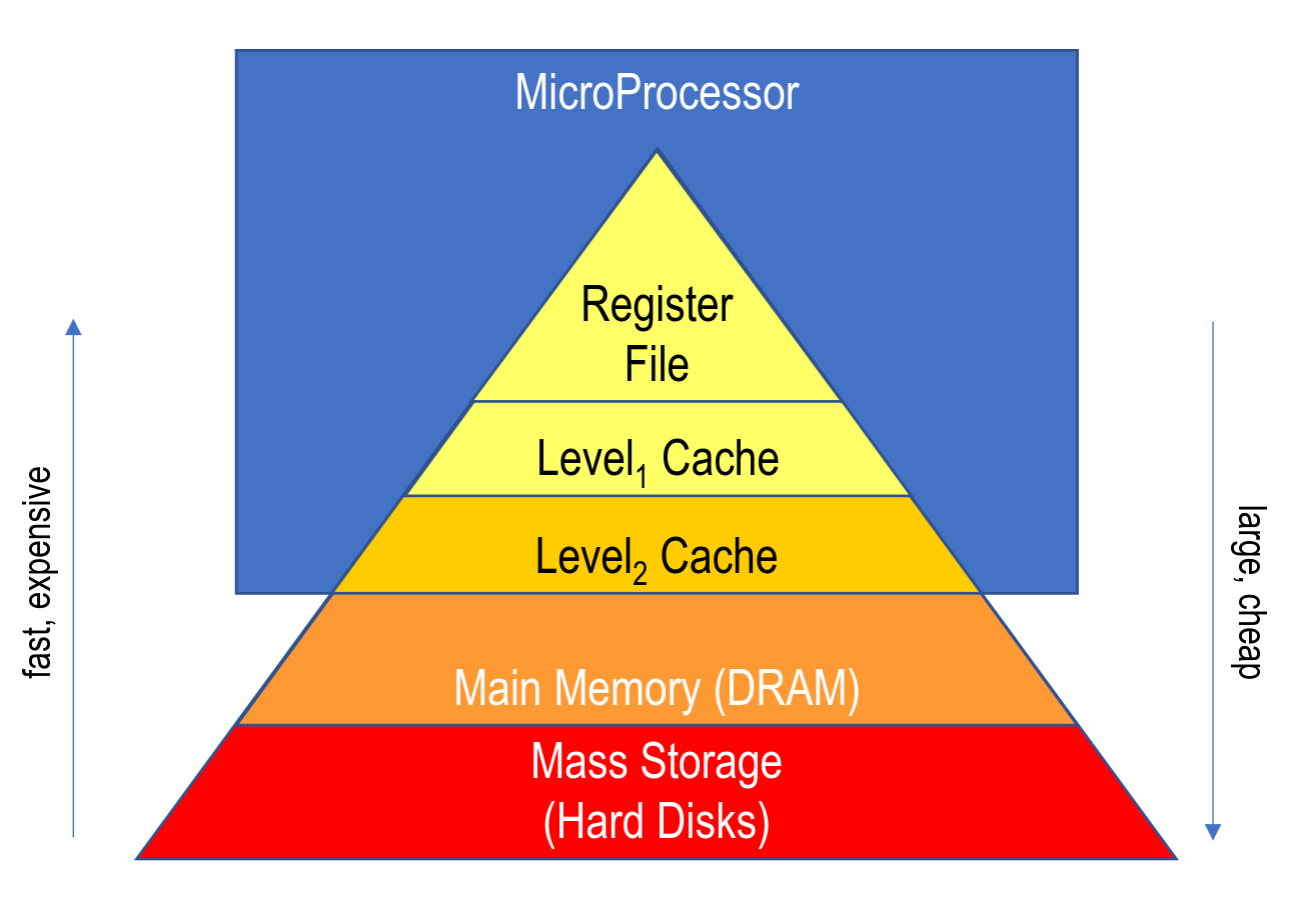
\includegraphics[scale=0.2]{../figures/cachy.png}
\end{center}

At this point we note that if SRAM is small, it becomes cheap, so there is some value in building a hierarchy of different memories to get high performance at low cost.
\begin{itemize}
	\item Expensive (and fast) memories should be used to store little, frequently accessed data. An SRAM is a great fit for this; 
	\item Cheap (and slow) memories should be used to store the bulk of the data. DRAMs is also a great fit for this.
\end{itemize}

Note that the computing system should not be aware of the differences: it simply sees a large, fast and cheap memory.

A clear problem is that data in the large DRAM does not fit into the small SRAM.
As we said, we intend to keep fractions of the DRAM in cache.
To maximize the use of the cache, we should ideally predict the data that is required next, and transfer it from DRAM in cache before it is needed.

\subsubsection{Hits and misses}

We refer by \textbf{MISS} to the situation where data is queried but not present in cache, and by \textbf{HIT} to the situation where data is queried and indeed present in cache.

\begin{itemize}
	\item For a MISS we have to check both the cache and the DRAM for actual data, so the total time the read operation takes is:
$$
t_\text{MISS} = t_\text{cache} + t_\text{DRAM}
$$
	\item For a HIT we have to check only the cache, so the total time the read operation takes is:
$$
t_\text{HIT} = t_\text{cache}
$$
\end{itemize}

By defining the hit rate $H$ as:
$$
H = \frac{n_\text{HIT}}{n_\text{TOT}}
$$

We get that the average time is:
$$
t_\text{avg} = H t_\text{HIT} + (1 - H) t_\text{MISS}
= H t_\text{cache} + (1 - H) (t_\text{cache} + t_\text{DRAM}) 
$$

Clearly, higher $H$ is better.

\subsubsection{Predictions}

To (somewhat) accurately predict the data that the microprocessor will need we exploit \textbf{locality} of data. 
There are 2 types of locality:
\begin{itemize}
	\item \textbf{Temporal} locality: the same data is used more often if it was recently referenced;
	\item \textbf{Spatial} locality: data around the data which was just used is more likely to be used next. 
\end{itemize}

\textit{Instructions}, for instnace, fit exactly in this framework as they are highly local (if we fetch instruction at \texttt{0x12} we will likely fetch at \texttt{0x16} next, assuming 32 bit instructions).

\subsubsection{Cache performance}

Let's talk about performance.
A large cache potentially makes execution faster, and if more data fits in the cache, the HIT Rate is higher.
Once all code and data is in cache we see no improvement in making the cache even larger.

Also, large memories are slower, with higher parasitic capacitances (meaning higher $t_\text{cache}$).
Checking cache for data takes time, and large memories consume more power.

A large cache is also more expensive, and the cost is additional to the large DRAM.

This makes cache sizing a trade-off between costs and performance, which is often application dependent.

\subsubsection{Cache policy}

Let's look at how actual cache systems are structured.

\begin{center}
	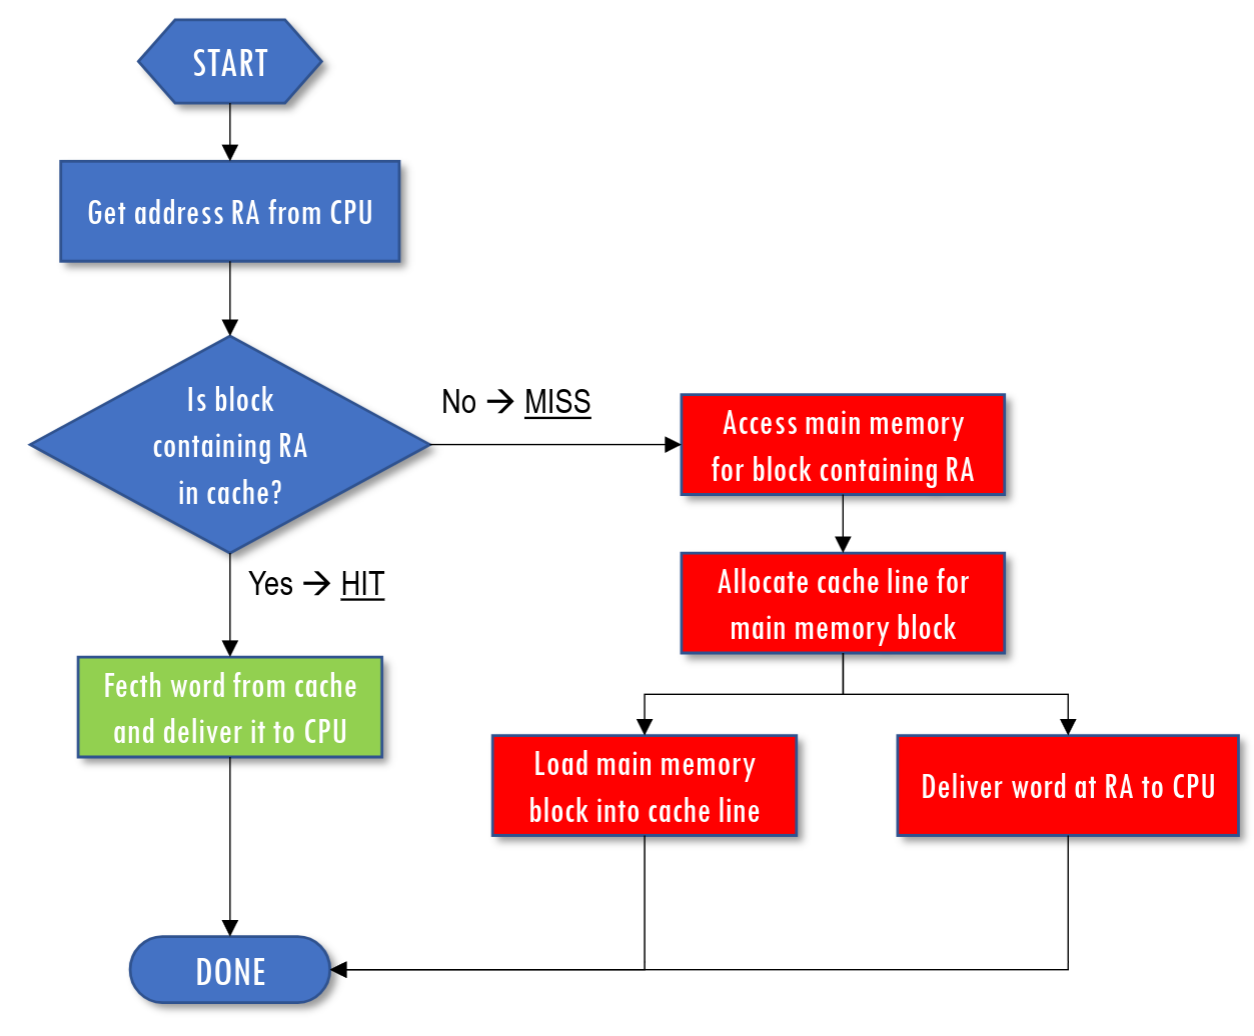
\includegraphics[scale=0.22]{../figures/cache_pol.png}
\end{center}

First we introduce the idea of a minimum unit of storage in cache, that is the \textbf{cache line}.
Data in DRAM is divided in \textbf{blocks}, with each block the same size of a cache line.
Blocks are aligned to the cache line size, and data is always moved to and from the cache in blocks.

At this point the microprocessor generates a main memory address, called \textbf{RA} (\textit{Read Address}). Of course, he word at RA belongs to a certain block.

If that word is in cache (that is, in a certain cacheline), we have to note addresses in DRAM and cache are different.
This means we need to find a fast way of knowing whether a given main memory block is alread stored in cache or not, and where.

The required data is identified by its address \(RA\) in main memory. Since data is transferred between main memory and cache in blocks, we can identify each block using its block address \(BA\), obtained from \(RA\). To determine whether a block is already present in the cache, we can use a \textit{Content-Addressable Memory} (CAM), in addition to the SRAM used to store the actual data. The CAM contains one entry per cache line, storing the corresponding main memory block address \(BA\), or just enough of it to identify the block. When a memory access occurs, the processor computes \(BA\) from \(RA\) and searches for a matching entry in the CAM. If a match is found, we have a \textit{cache hit}: the CAM identifies the corresponding cache line, allowing the requested word to be retrieved from SRAM. Otherwise, we have a \textit{cache miss}: the block is fetched from DRAM, stored in a cache line, and its address is recorded in the CAM. The requested word can then be returned to the processor.

This is usually referred to as \textit{fully associative} caches.
We'll see that it's not the only approach.

\end{document}
